\section{Appendix: MVA Correlations}
\label{app:mvacorr}

Since we use a complete set of minimum number of 
input variables necessary to describe the whole event topology, 
these variables are mostly mostly uncorrelated. 
The correlation matrix for signal and background 
samples are shown in Figs~\ref{fig:FigCorr170Mu}--\ref{fig:FigCorr600Mu}
for all Higgs mass points.
%%%%%%%%%%%%%%%%%%%
\subsection{Correlation matrix: \texorpdfstring{$M_H$}{M(H)} = 170~GeV}
%%%%%%%%%%%%%%%%%%%
\begin{figure}[bthp!]
\subfigure[]{
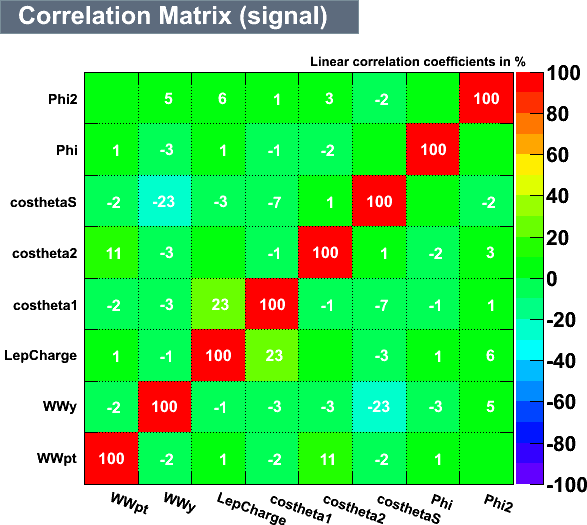
\includegraphics[width=0.49\textwidth]{plots/2012_MVA/TMVA_170_nJ2_mu_CorrelationMatrixS}
}
\subfigure[]{
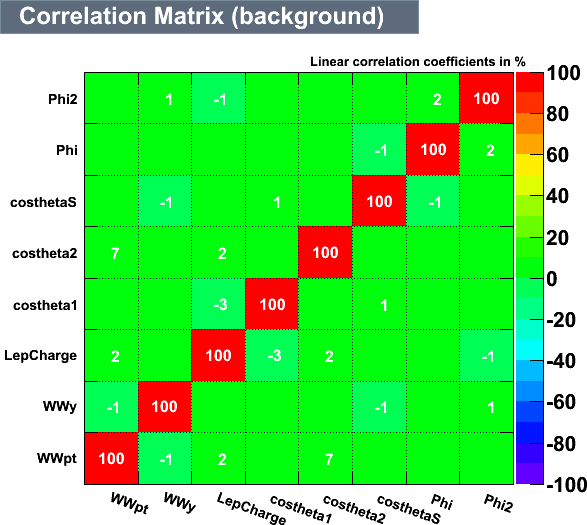
\includegraphics[width=0.49\textwidth]{plots/2012_MVA/TMVA_170_nJ2_mu_CorrelationMatrixB}
}
\caption{\label{fig:FigCorr170Mu} 
Input correlation matrix for $M_H =$170 GeV: (a) signal, (b) W+jets background 
}
\end{figure}
%%%%%%%%%%%%%%%%%%%
\subsection{Correlation matrix: \texorpdfstring{$M_H$}{M(H)} = 180~GeV}
%%%%%%%%%%%%%%%%%%%
\begin{figure}[bthp!]
\subfigure[]{
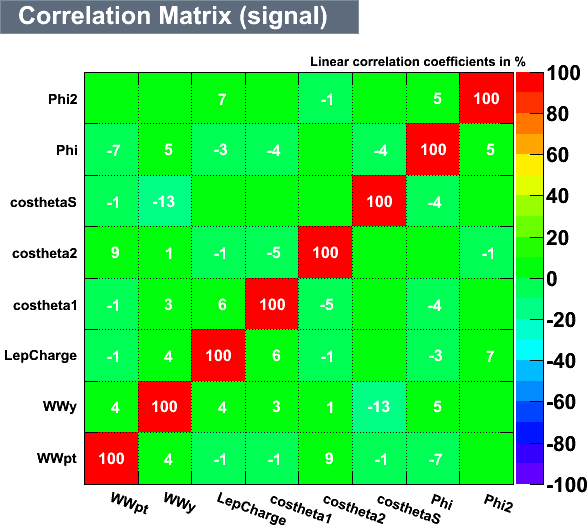
\includegraphics[width=0.49\textwidth]{plots/2012_MVA/TMVA_180_nJ2_mu_CorrelationMatrixS}
}
\subfigure[]{
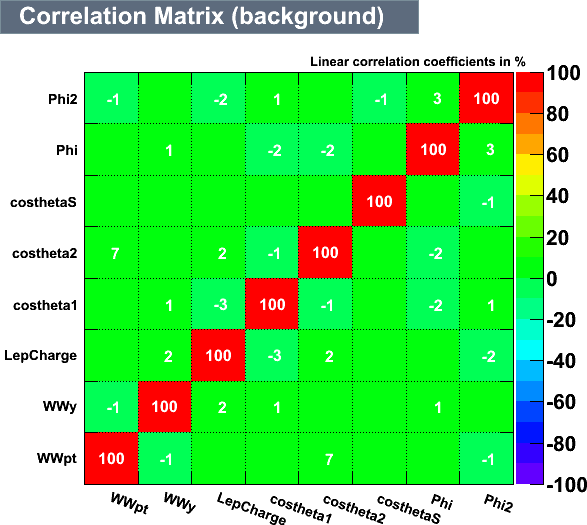
\includegraphics[width=0.49\textwidth]{plots/2012_MVA/TMVA_180_nJ2_mu_CorrelationMatrixB}
}
\caption{\label{fig:FigCorr180Mu} 
Input correlation matrix for $M_H =$180 GeV: (a) signal, (b) W+jets background 
}
\end{figure}
%%%%%%%%%%%%%%%%%%%
\newpage
\subsection{Correlation matrix: \texorpdfstring{$M_H$}{M(H)} = 190~GeV}
%%%%%%%%%%%%%%%%%%%
\begin{figure}[bthp!]
\subfigure[]{
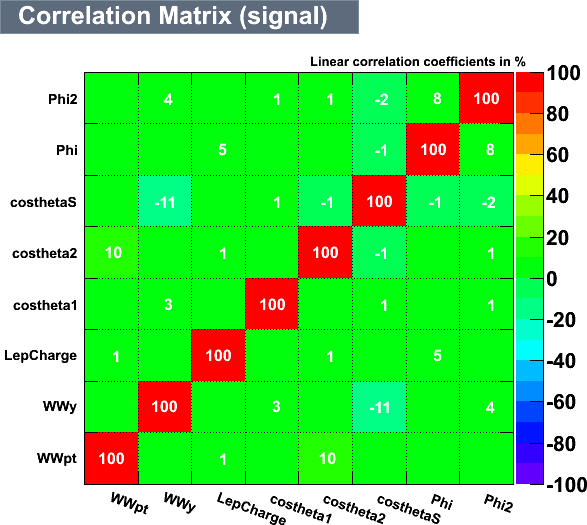
\includegraphics[width=0.49\textwidth]{plots/2012_MVA/TMVA_190_nJ2_mu_CorrelationMatrixS}
}
\subfigure[]{
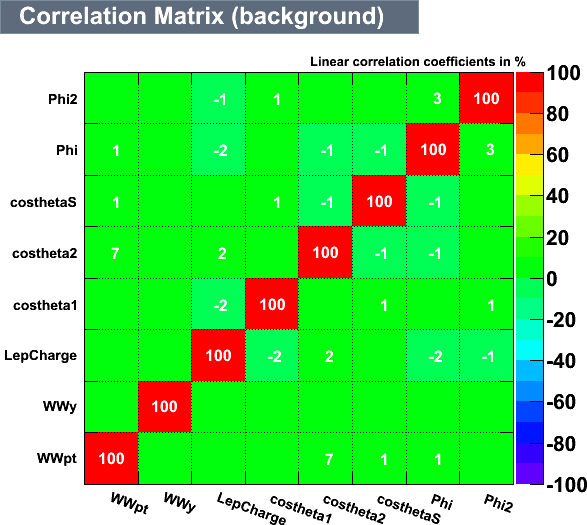
\includegraphics[width=0.49\textwidth]{plots/2012_MVA/TMVA_190_nJ2_mu_CorrelationMatrixB}
}
\caption{\label{fig:FigCorr190Mu} 
Input correlation matrix for $M_H =$190~GeV: (a) signal, (b) W+jets background 
}
\end{figure}
%%%%%%%%%%%%%%%%%%%
\subsection{Correlation matrix: \texorpdfstring{$M_H$}{M(H)} = 200~GeV}
%%%%%%%%%%%%%%%%%%%
\begin{figure}[bthp!]
\subfigure[]{
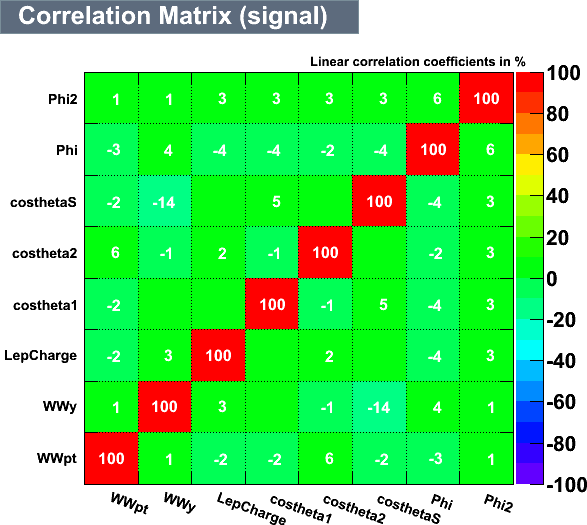
\includegraphics[width=0.49\textwidth]{plots/2012_MVA/TMVA_200_nJ2_mu_CorrelationMatrixS}
}
\subfigure[]{
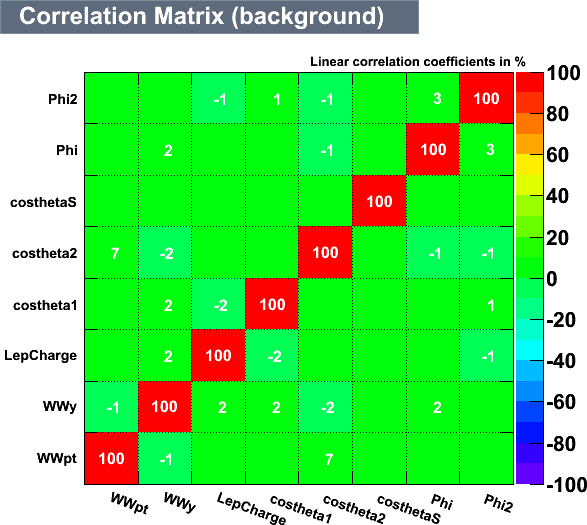
\includegraphics[width=0.49\textwidth]{plots/2012_MVA/TMVA_200_nJ2_mu_CorrelationMatrixB}
}
\caption{\label{fig:FigCorr200Mu} 
Input correlation matrix for $M_H =$200~GeV: (a) signal, (b) W+jets background 
}
\end{figure}
%%%%%%%%%%%%%%%%%%%
\newpage
\subsection{Correlation matrix: \texorpdfstring{$M_H$}{M(H)} = 250~GeV}
%%%%%%%%%%%%%%%%%%%
\begin{figure}[bthp!]
\subfigure[]{
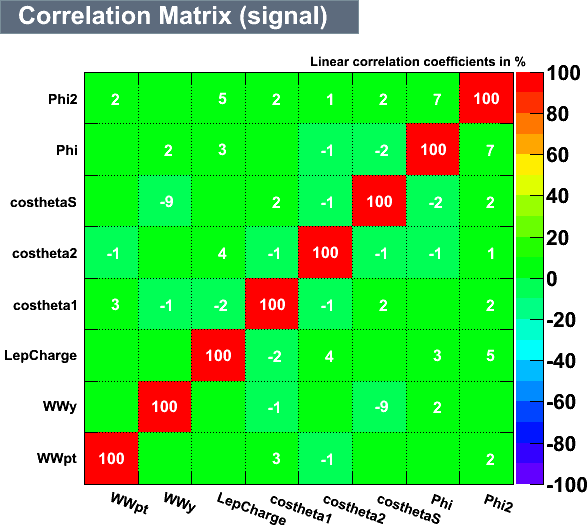
\includegraphics[width=0.49\textwidth]{plots/2012_MVA/TMVA_250_nJ2_mu_CorrelationMatrixS}
}
\subfigure[]{
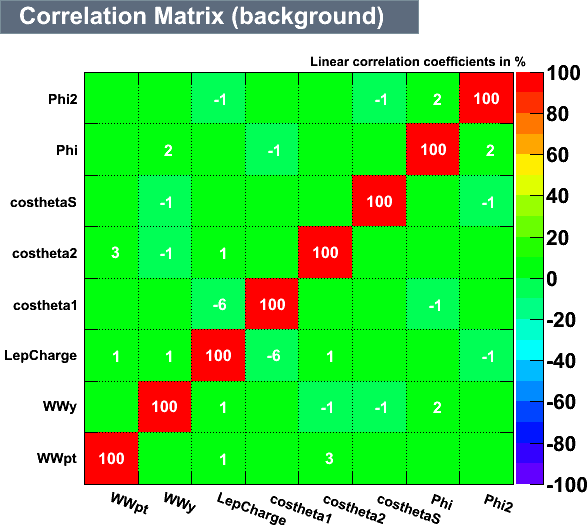
\includegraphics[width=0.49\textwidth]{plots/2012_MVA/TMVA_250_nJ2_mu_CorrelationMatrixB}
}
\caption{\label{fig:FigCorr250Mu} 
Input correlation matrix for $M_H =$250~GeV: (a) signal, (b) W+jets background 
}
\end{figure}
%%%%%%%%%%%%%%%%%%%
\subsection{Correlation matrix: \texorpdfstring{$M_H$}{M(H)} = 300~GeV}
%%%%%%%%%%%%%%%%%%%
\begin{figure}[bthp!]
\subfigure[]{
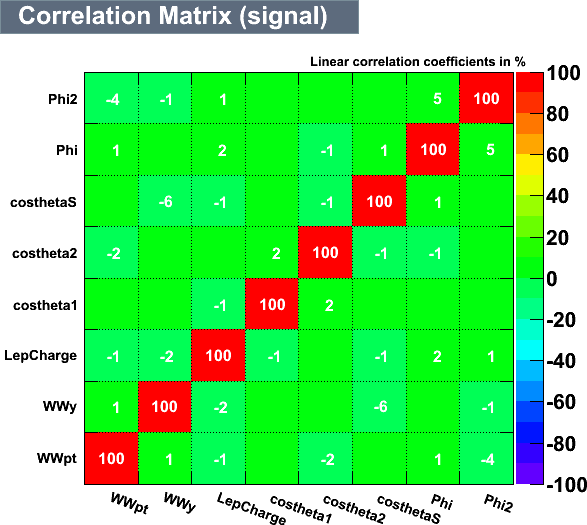
\includegraphics[width=0.49\textwidth]{plots/2012_MVA/TMVA_300_nJ2_mu_CorrelationMatrixS}
}
\subfigure[]{
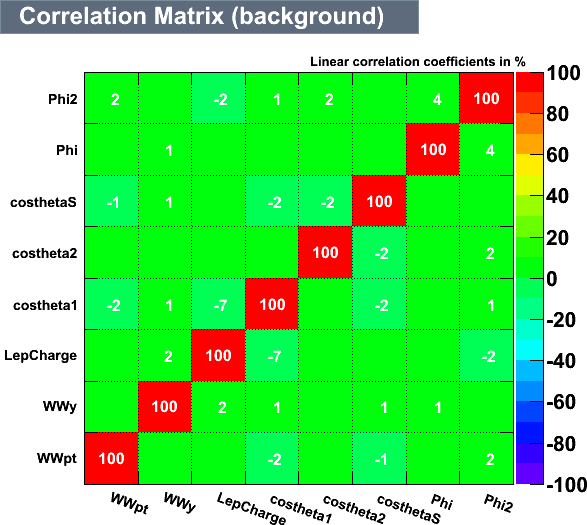
\includegraphics[width=0.49\textwidth]{plots/2012_MVA/TMVA_300_nJ2_mu_CorrelationMatrixB}
}
\caption{\label{fig:FigCorr300Mu} 
Input correlation matrix for $M_H =$300~GeV: (a) signal, (b) W+jets background 
}
\end{figure}
%%%%%%%%%%%%%%%%%%%
\newpage
\subsection{Correlation matrix: \texorpdfstring{$M_H$}{M(H)} = 350~GeV}
%%%%%%%%%%%%%%%%%%%
\begin{figure}[bthp!]
\subfigure[]{
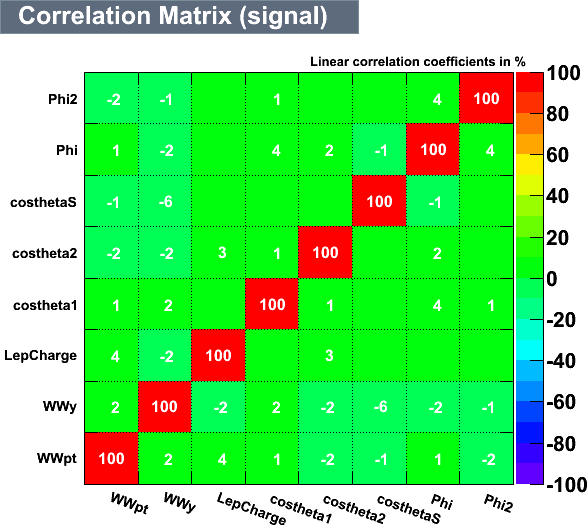
\includegraphics[width=0.49\textwidth]{plots/2012_MVA/TMVA_350_nJ2_mu_CorrelationMatrixS}
}
\subfigure[]{
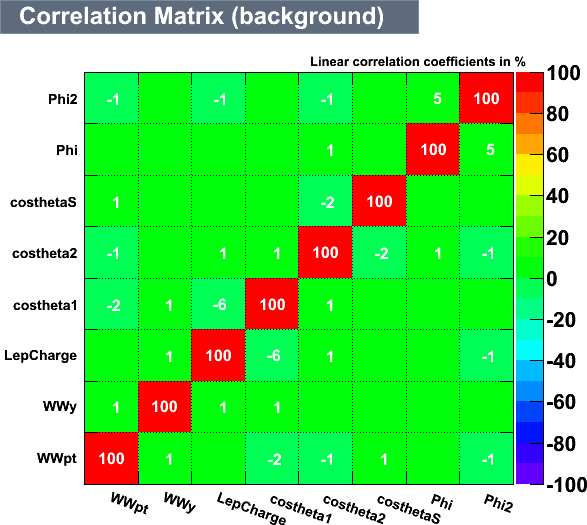
\includegraphics[width=0.49\textwidth]{plots/2012_MVA/TMVA_350_nJ2_mu_CorrelationMatrixB}
}
\caption{\label{fig:FigCorr350Mu} 
Input correlation matrix for $M_H =$350~GeV: (a) signal, (b) W+jets background 
}
\end{figure}
%%%%%%%%%%%%%%%%%%%
\subsection{Correlation matrix: \texorpdfstring{$M_H$}{M(H)} = 400~GeV}
%%%%%%%%%%%%%%%%%%%
\begin{figure}[bthp!]
\subfigure[]{
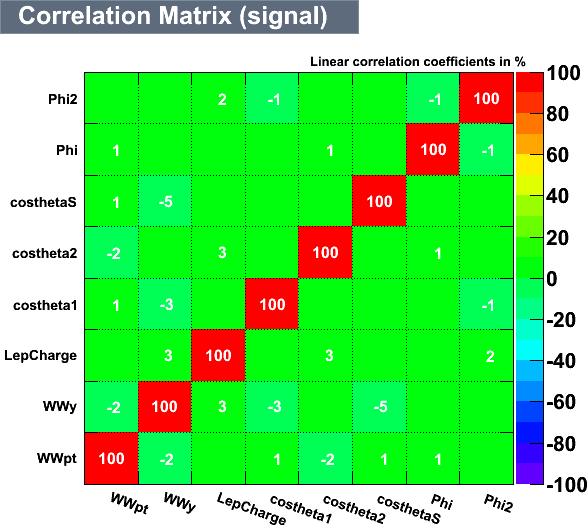
\includegraphics[width=0.49\textwidth]{plots/2012_MVA/TMVA_400_nJ2_mu_CorrelationMatrixS}
}
\subfigure[]{
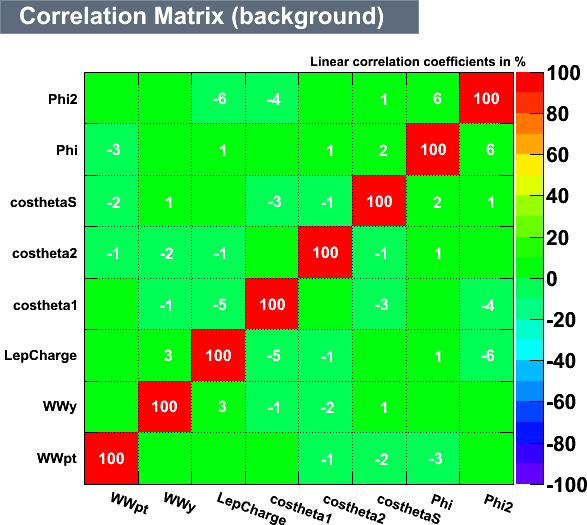
\includegraphics[width=0.49\textwidth]{plots/2012_MVA/TMVA_400_nJ2_mu_CorrelationMatrixB}
}
\caption{\label{fig:FigCorr400Mu} 
Input correlation matrix for $M_H =$400~GeV: (a) signal, (b) W+jets background 
}
\end{figure}
%%%%%%%%%%%%%%%%%%%
\newpage
\subsection{Correlation matrix: \texorpdfstring{$M_H$}{M(H)} = 450~GeV}
%%%%%%%%%%%%%%%%%%%
\begin{figure}[bthp!]
\subfigure[]{
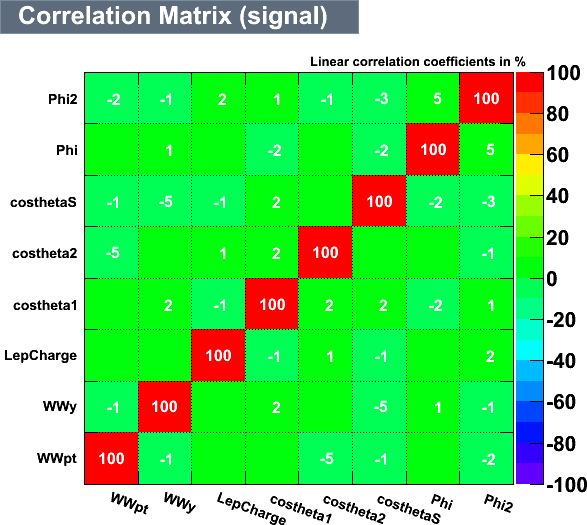
\includegraphics[width=0.49\textwidth]{plots/2012_MVA/TMVA_450_nJ2_mu_CorrelationMatrixS}
}
\subfigure[]{
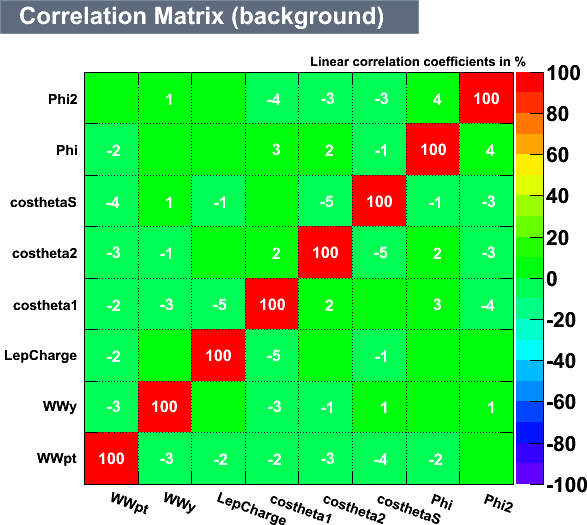
\includegraphics[width=0.49\textwidth]{plots/2012_MVA/TMVA_450_nJ2_mu_CorrelationMatrixB}
}
\caption{\label{fig:FigCorr450Mu} 
Input correlation matrix for $M_H =$450~GeV: (a) signal, (b) W+jets background 
}
\end{figure}
%%%%%%%%%%%%%%%%%%%
\subsection{Correlation matrix: \texorpdfstring{$M_H$}{M(H)} = 500~GeV}
%%%%%%%%%%%%%%%%%%%
\begin{figure}[bthp!]
\subfigure[]{
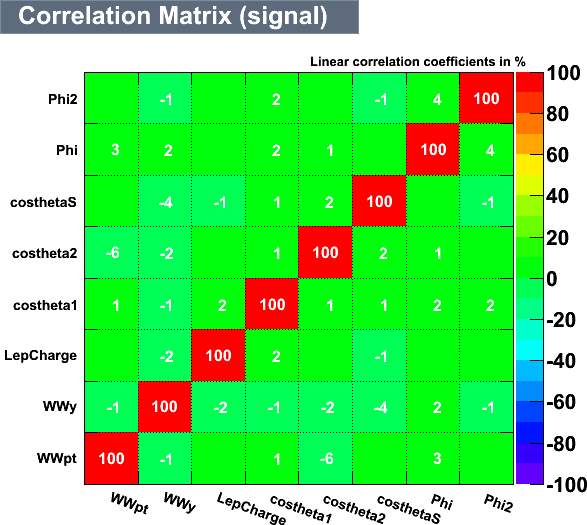
\includegraphics[width=0.49\textwidth]{plots/2012_MVA/TMVA_500_nJ2_mu_CorrelationMatrixS}
}
\subfigure[]{
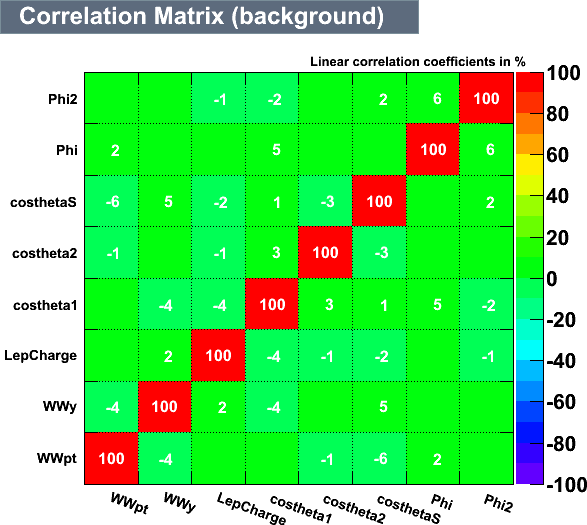
\includegraphics[width=0.49\textwidth]{plots/2012_MVA/TMVA_500_nJ2_mu_CorrelationMatrixB}
}
\caption{\label{fig:FigCorr500Mu} 
Input correlation matrix for $M_H =$500~GeV: (a) signal, (b) W+jets background 
}
\end{figure}
%%%%%%%%%%%%%%%%%%%
\newpage
\subsection{Correlation matrix: \texorpdfstring{$M_H$}{M(H)} = 550~GeV}
%%%%%%%%%%%%%%%%%%%
\begin{figure}[bthp!]
\subfigure[]{
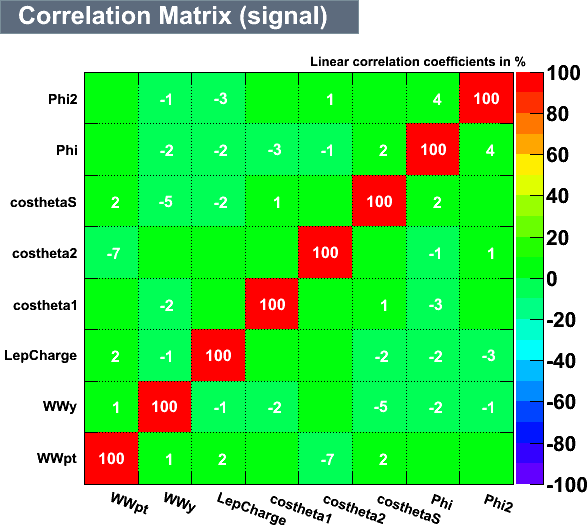
\includegraphics[width=0.49\textwidth]{plots/2012_MVA/TMVA_550_nJ2_mu_CorrelationMatrixS}
}
\subfigure[]{
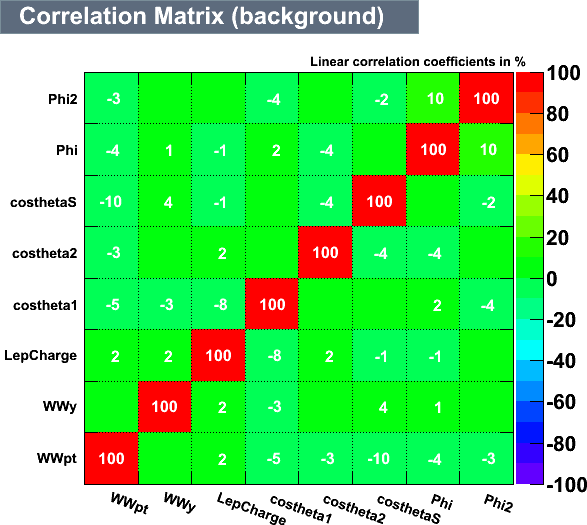
\includegraphics[width=0.49\textwidth]{plots/2012_MVA/TMVA_550_nJ2_mu_CorrelationMatrixB}
}
\caption{\label{fig:FigCorr550Mu} 
Input correlation matrix for $M_H =$550~GeV: (a) signal, (b) W+jets background 
}
\end{figure}
%%%%%%%%%%%%%%%%%%%
\subsection{Correlation matrix: \texorpdfstring{$M_H$}{M(H)} = 600~GeV}
%%%%%%%%%%%%%%%%%%%
\begin{figure}[bthp!]
\subfigure[]{
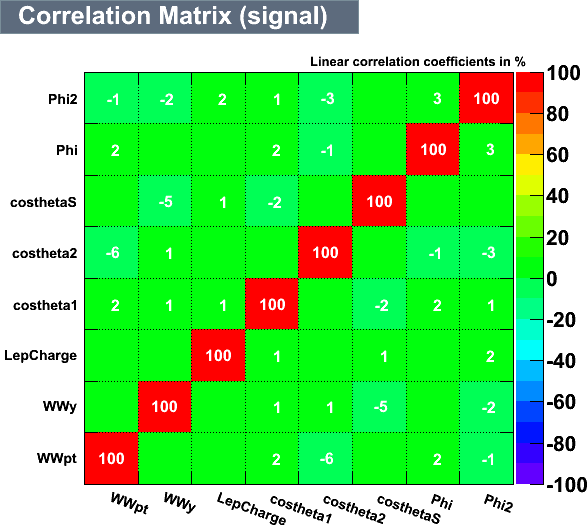
\includegraphics[width=0.49\textwidth]{plots/2012_MVA/TMVA_600_nJ2_mu_CorrelationMatrixS}
}
\subfigure[]{
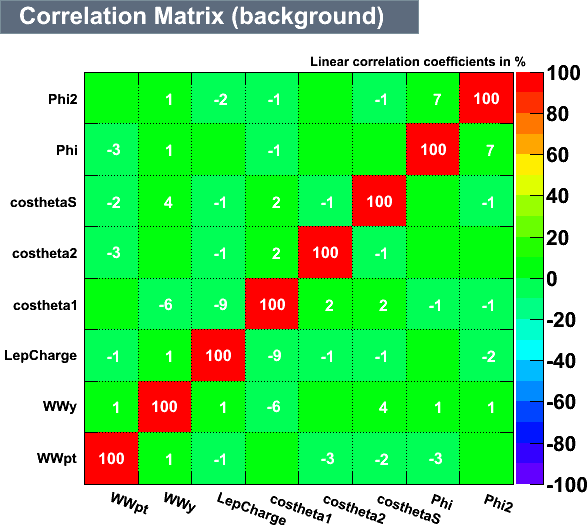
\includegraphics[width=0.49\textwidth]{plots/2012_MVA/TMVA_600_nJ2_mu_CorrelationMatrixB}
}
\caption{\label{fig:FigCorr600Mu} 
Input correlation matrix for $M_H =$600~GeV: (a) signal, (b) W+jets background 
}
\end{figure}
%%%%%%%%%%%%%%%%%%%
